\documentclass[conference]{IEEEtran}
\IEEEoverridecommandlockouts
% The preceding line is only needed to identify funding in the first footnote. If that is unneeded, please comment it out.
\usepackage{cite}
\usepackage{amsmath,amssymb,amsfonts}
\usepackage{algorithmic}
\usepackage{graphicx}
\usepackage{hyperref}
\usepackage{textcomp}
\usepackage{xcolor}
\usepackage{listings}
\usepackage{tabularx}



\newcommand{\todo}[1]{\textcolor{red}{{\bfseries [[#1]]}}}
\def\BibTeX{{\rm B\kern-.05em{\sc i\kern-.025em b}\kern-.08em
    T\kern-.1667em\lower.7ex\hbox{E}\kern-.125emX}}
\begin{document}

\title{Do Automated Fault Localization Techniques Work For REST APIs?}

\author{\IEEEauthorblockN{Aakash Kulkarni}
\IEEEauthorblockA{\textit{School of EECS} \\ % --- To do ---
\textit{Oregon State University}\\ % --- To do ---
Corvallis, United States \\ % --- To do ---
kulkaraa@oregonstate.edu}
\and
\IEEEauthorblockN{Soon Song Cheok}
\IEEEauthorblockA{\textit{School of EECS} \\ % --- To do ---
\textit{Oregon State University}\\ % --- To do ---
Corvallis, United States \\ % --- To do ---
cheoks@oregonstate.edu}
\and
\IEEEauthorblockN{Shreyes Joshi}
\IEEEauthorblockA{\textit{School of EECS} \\ % --- To do ---
\textit{Oregon State University}\\ % --- To do ---
Corvallis, United States \\ % --- To do ---
joshish@oregonstate.edu}
}

\maketitle

\begin{abstract}

\end{abstract}

\begin{IEEEkeywords}

\end{IEEEkeywords}


\section{Introduction}
\label{sec:introduction}

% \subsection{Problem statement}
    REST APIs (Representational State Transfer) have become backbone of the modern web and cloud applications. They facilitate seamless interactions between client and server through stateless communication, enabling services to be scalable, reliable, and easily integrateable ~\cite{li2016} ~\cite{neumann2018}. Basically, REST APIs are a set of rules and standards  defined by OpenAPI ~\cite{ed-douibi2018} used to enable communication between different software applications over the internet. They are built around the use of standard HTTP methods such as GET, POST, PUT, and DELETE to interact with resources, which are any kind of data or service that can be named on a network.
    Given their critical role, the effective identification and resolution of faults within REST APIs remain a significant challenge ~\cite{barbir2007}, prompting the need for research on how fault localization techniques work to their unique structure and functionality.

    % \todo{What is the problem statement that you plan to solve?}

% \subsection{Motivation}
    As systems that rely on REST APIs grow in scale and complexity  ~\cite{khare2004} , minor faults can escalate into major disruptions, impacting user experience and business operations. 
    This research is motivated by the need to evaluate how well current fault localization techniques perform in the unique context of REST APIs. 
    The goal is to determine if these techniques can indeed be applied effectively to REST APIs and, if so, to explore which types of faults are more amenable to being localized. 
    This understanding could potentially allow developers to more efficiently diagnose and address issues, thereby enhancing the stability and performance of REST API-based systems.


    % \todo{Why should anyone care about solving that problem?}

% \subsection{Relation with software engineering research}

    Fault localization is a well-established area of research within software engineering, traditionally concentrated on more conventional software systems. 
    REST APIs, however, present distinct challenges that complicate fault localization due to their composition and operational dynamics. 
    Additionally, the architecture of REST APIs often involves diverse artifacts that are not source code, such as configuration files, API specifications, and database schemas.


    % \todo{How is the problem related to software engineering research? What is already known about that problem space, and what is still unknown that you are interested in solving?}

% \subsection{Key Insight or Idea}
    The primary objective of this research is to evaluate the effectiveness of existing fault localization techniques within the unique context of REST APIs, which feature a mix of code and non-code artifacts. 
    This study will systematically apply established fault localization methods like BLUES ~\cite{ManishBluesFaultLocalization} and LLMAO ~\cite{LLMAOFaultLocalization} to a dataset of REST API faults. 
    This dataset will be meticulously developed to represent a wide range of faults typical in REST APIs and classified according to an existing comprehensive taxonomy derived from previous research.

    This approach will enable us to assess the applicability of these fault localization techniques to REST APIs by determining how effectively they can identify and localize different types of faults. 
    % Importantly, this research does not assume the prior effectiveness of these techniques in REST API contexts but seeks to establish empirical evidence of their performance. 
    The analysis will provide insights into whether traditional fault localization methods are suited to the complexities of REST APIs, especially considering their unique structural and functional characteristics.


    % \todo{What is the high-level approach that you would like to explore to solve the problem? Why you feel you can succeed with that approach in 5 weeks?}

% \subsection{Assumptions}
    Our assumptions:
    \begin{itemize}
        % \item \textit{Assumption 1:} It is assumed that the faults in the dataset are correctly classified according to the existing comprehensive taxonomy ~\cite{automatedTestTaxonomy} .
        \item \textit{Assumption:} Assume that the selected fault localization techniques are suitable for application to REST APIs, despite their original design for conventional software systems. This includes the assumption that these techniques can handle the unique challenges posed by REST APIs, such as dealing with non-code artifacts.
    \end{itemize}

    % \todo{What kind of assumptions will you need to make for your choice of solution?}

% \subsection{Research questions}
    The primary research questions are formulated as follows:
    \begin{itemize}
        \item \textbf{RQ1:} What categories of faults are most effectively localized by current techniques?
        \item \textbf{RQ2:} Which fault localization technique is highly effective in the context of REST APIs?
    \end{itemize}
    % \todo{What research question(s) will you answer?}

% \subsection{Evaluation Dataset}
For the evaluation dataset, we will manually select the issues from the GitHub services and their fixes from REST API projects that utilize Spring Boot or Jersey frameworks. These GitHub services are used in the paper  \textit{Generating REST API Specifications through Static Analysis} by Manish et al ~\cite{ManishRestServices}
This dataset will encompass various categories of faults identified in REST APIs. By analyzing repositories and commit histories, we will extract specific instances where bugs have been documented and subsequently fixed. 
The categorization of these faults will be categorized with an established taxonomy of API faults ~\cite{automatedTestTaxonomy} , ensuring that each bug is classified according to its nature and impact. This rigorous dataset compilation aims to provide a comprehensive basis for testing fault localization techniques within a controlled, relevant environment.

% \subsection{Evaluation metrics}
For evaluation of fault localization techniques using the dataset derived from REST APIs employing Spring Boot and Jersey frameworks will be measured by Top-k accuracy, and EXAM score.
These metrics will collectively provide a thorough assessment of each fault localization technique's ability to detect and accurately categorize faults in REST APIs, contributing to a detailed understanding of their practical utility and areas for improvement.

    % \todo{How will you know that you have solved the problem successfully? In other words, how will you evaluate your solution?}


\section{Background and Motivation}
\label{sec:background-and-motivation}

\subsection{Importance of REST APIs}

REST APIs (Representational State Transfer APIs) are central to modern web and cloud applications, serving as critical conduits for data exchange and system integration. 
They leverage standard HTTP methods like GET, POST, PUT, and DELETE to interact with networked resources, making them integral to the architecture of distributed systems. 
The scalability, reliability, and ease of integration provided by REST APIs facilitate seamless interactions between clients and servers, thereby enhancing the performance and flexibility of complex software ecosystems. 
Their widespread adoption underscores their importance in today's technology landscape, where rapid communication and data accessibility are paramount.

\subsection{Challenges of Fault Localization in REST APIs}
While REST APIs have simplified the development and management of modern applications, they introduce specific challenges that complicate fault localization.
The architecture often involves non-code artifacts such as API specifications, configuration files, and database schemas, which are not traditionally addresses by fault localization techniques developed for code-centric applications. 


\subsection{Gaps in Current Research}
Fault localization is a well-established research area within software engineering, focusing primarily on identifying the locations of faults in conventional software systems to reduce debugging time and enhance system reliability.
 However, the unique operational dynamics and architectural complexities of REST APIs pose new challenges that are not fully addressed by existing fault localization techniques.
Previous studies have developed fault taxonomies for REST APIs which are helpful if the FL techniques can localize faults to understand what categories of faults can be localized.
There remains a significant knowledge gap regarding the effectiveness of these techniques in accurately identifying and localizing faults in REST APIs, particularly those involving non-code artifacts.


\subsection{Need for Targeted Research on Fault Localization in REST APIs}
This research is motivated by the critical need to evaluate and understand the performance of existing fault localization techniques within the REST API context. 
By determining how effectively these techniques can identify and localize faults in REST APIs, developers can gain valuable insights that could lead to quicker and more accurate fault diagnosis. This is particularly important as even minor faults can escalate into major disruptions in REST API-dependent systems, affecting user experience and operational efficiency. Addressing this gap will not only contribute to the field by enhancing the robustness and reliability of REST APIs but also by supporting the development of more sophisticated tools and methodologies tailored to the needs of modern software architectures.


\subsection{Research Objectives}
The primary objective of this research is to systematically assess the applicability of established fault localization techniques—namely 
BLUES and LLMAO to a curated dataset of REST API faults. 
This dataset will be developed to encompass a broad spectrum of typical faults in REST APIs and will be classified according to an existing comprehensive taxonomy. 
The insights gained from this study are expected to reveal whether traditional fault localization methods are suitable for the complex environments of REST APIs and may guide future efforts in refining these techniques or developing new approaches specifically designed for REST API ecosystems.

\begin{figure*}[t] 
    \centering
    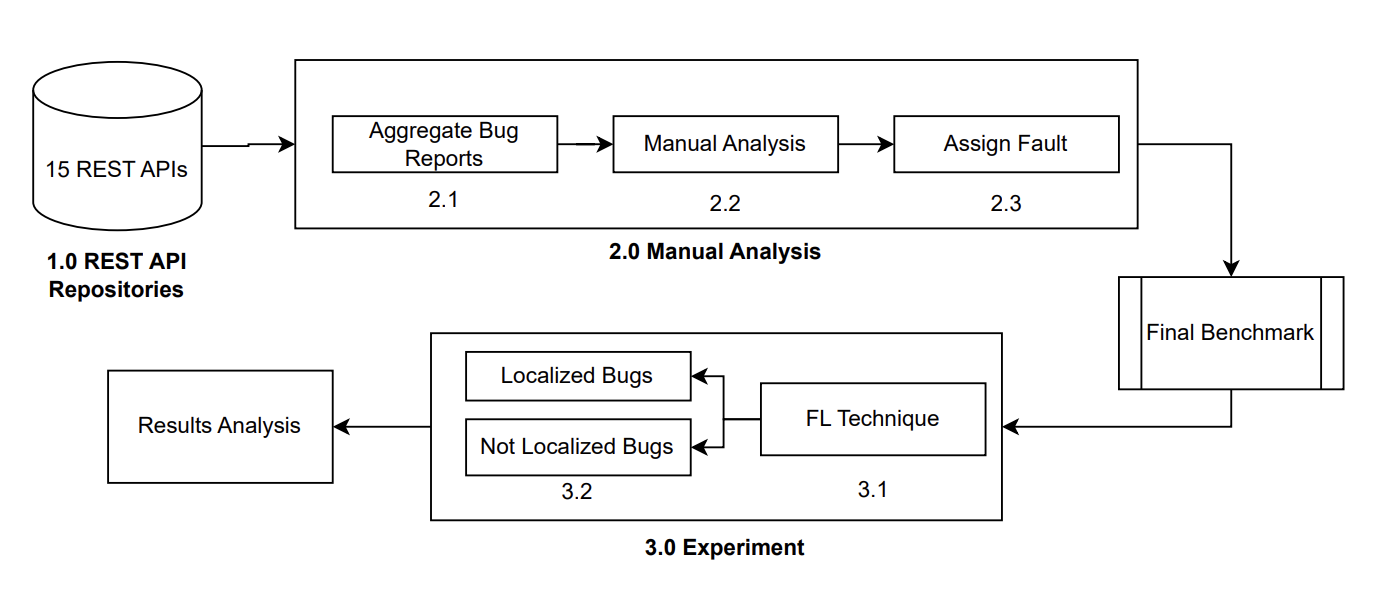
\includegraphics[width=1.0\textwidth]{fig2.png}
    \caption{Approach Overview}
    \label{fig:widefigure}
  \end{figure*}

\section{Related Work}
\label{sec:relatedwork}

Fault localization techniques have long been an integral part of software maintenance, aiding developers by pinpointing the origins of failures within software systems. 
A variety of approaches have been explored ~\cite{Wong2023_Software_Fault_localization}, including Information Retrieval (IR) based methods, Spectrum-Based Fault Localization (SFL), and more comprehensive software engineering tools.

Information Retrieval Based Fault Localization: The work by Klaus Changsun Youm et al introduces an advanced IR-based fault localization method called BLIA, which integrates bug reports and code change history to enhance the localization process  ~\cite{7467300} ~\cite{ctx114059874780001451}. BLIA notably improves the accuracy of locating bugs by analyzing texts, stack traces, and comments within bug reports alongside source file structures and version histories. This method has shown significant improvements over previous tools such as BugLocator and BLUiR, particularly at the file and method levels, by refining the granularity of localization results. This approach underscores the potential of IR-based methods in handling complex software systems, aligning with the need to explore such techniques within REST API environments.

The Jaguar tool, described by Ribeiro et al, utilizes SBFL technique to identify faulty code excerpts in Java programs ~\cite{8367068}. By employing both control-flow and data-flow spectra and integrating the lightweight ba-dua coverage tool, Jaguar efficiently supports the analysis of large programs. The capability of Jaguar to provide detailed visualizations of suspicious program elements highlights the effectiveness of SFL in traditional software environments. The distinction between data-flow and control-flow spectra offers a nuanced view of fault localization that could be pertinent to analyzing REST APIs, known for their complex interactions and stateless operations.

Debugging in IDEs, particularly using tools like Visual Studio Code for web applications, illustrates the practical aspects of fault localization in real-world scenarios ~\cite{DebuggingCode}. The capabilities of IDEs to facilitate debugging through breakpoints and variable inspections are directly relevant to the challenges faced in REST API development, where faults may not only arise from code but also from API configurations and interactions.





\section{Approach}
\label{sec:approach}

\subsection{Dataset Creation and Preparation}

To effectively assess the applicability of fault localization techniques to REST APIs, In our research, we utilize a set of REST API services previously employed in the study "Generating REST API Specifications through Static Analysis" by Manish et al ~\cite{ManishRestServices}. These services are chosen due to their diverse characteristics and well-documented configurations, making them suitable subjects for evaluating fault localization techniques. 
The faults from these services will be categorized based on a previously established taxonomy of REST API faults, ensuring that each fault type is adequately represented. We are three graduate students with knowledge on REST API, we have selected the issues on GitHub Repositories, and we have the read the messages of their issues and saw what were the changes made and given it a fault type. We all have gone through all the services and then we together consolidated into one single list where we found 26 Faults which we can test using the Fault Localization Techniques. 

\subsection{Selection of Fault Localization Techniques}

The study will focus on two primary fault localization techniques that have shown promise in traditional software contexts but whose effectiveness in REST APIs remains underexplored:
\begin{enumerate}
    \item \textbf{BLUES:} ~\cite{ManishBluesFaultLocalization} BLUES is developed by a group of researchers Manish et al which takes Bug report as input and generates the suspicious ranked list of faulty code.
    \item \textbf{LLMAO:} ~\cite{LLMAOFaultLocalization} LLMAO is developed by a group of researchers Aidan et al, where LLMAO is first LLM (Large Language Model) based for fault localization and which takes no inputs. But it finds the difference between two commits to see where the bug was introduced and creates a ranked list of faulty code. 

\end{enumerate}

Both the Fault Localization Techniques are known for their effective finding of the faulty code. And also both the techniques are new.

\subsection{Integration with REST API Characteristics}

Given the unique challenges posed by REST APIs, such as stateless operations and the presence of non-code artifacts (e.g., configuration files and API specifications), our approach will also consider these elements:
\begin{itemize}
    \item \textbf{Non-Code Artifacts}: Special attention will be given to faults that may originate from or affect non-code artifacts. 
\end{itemize}


\section{Evaluation}
\label{sec:evaluation}

\subsection{Dataset}
\label{sec:dataset}

To conduct this research, a dataset is required for evaluation. The dataset contains REST API faults, their sources, and other relevant information necessary like Bug Reports to evaluate FL techniques.

The dataset we started with had  GitHub APIs from 15 different REST API repositories from the services were management-api-for-apache-cassandra, catwatch, cwa-verification-server, digdag, enviroCar-server, features-service,
gravitee-api-management, kafka-rest, ocvn, ohsome-api, proxyprint-kitchen, quartz-manager, restcountries, senzing-api-server, and Ur-Codebin-API.
The  process of filtering out issues not marked as 'bugs' and 'closed,' leaving only the set of issues that have been fixed details ~\ref{tab:repositories}. Issues involving code changes are collected and then further filtered through manual analysis to select those applicable to this research. These services provide us services with bug information we need to create a benchmark on REST API faults.

\begin{table}
    \centering
    \caption{List of Repositories}
    \label{tab:repositories}
    \begin{tabular}{|c|l|c|}
    \hline
        \hline
        \textbf{No.} & \textbf{Repository Name} & \textbf{\# of Faults} \\ \hline
        1 & management-api-for-apache-cassandra & 2 \\ \hline
        2 & cwa-verification-server &  7 \\ \hline
        3 & digdag & 2 \\ \hline
        4 & ohsome-api & 10 \\ \hline
        5 & kafka-rest & 3 \\ \hline
    \end{tabular}
\end{table}
    




% The fault taxonomy had 4 Major fault types where each major fault type has sub-categories from ~\cite{automatedTestTaxonomy}, in total we had 19 categories of faults we can divide into. 

The fault taxonomy utilized in our study delineates four major fault types, each encompassing various sub-categories as outlined in ~\cite{automatedTestTaxonomy}. Collectively, these categories provide a comprehensive framework, dividing the faults into a total of 19 distinct categories. 
This detailed classification aids in systematically analyzing and categorizing the faults encountered during the testing of REST APIs to create the Table ~\ref{tab:faultData}


\begin{table}[ht]
    \centering
    \caption{Fault Data}
    \label{tab:faultData}
    \begin{tabular}{|c|p{6cm}|c|}
    \hline
        \hline
        \textbf{No.} & \textbf{Fault Type} & \textbf{\# of Faults} \\ \hline
        1 & DB Operations/ Optimistic Lock Exception & 1 \\ \hline
        2 & DB Operations/ Unique Index or Primary Key &  2 \\ \hline
        3 & Incomplete Specification/Form/Format & 1 \\ \hline
        4 & Framework Misconfiguration/ Rejected Calls & 2 \\ \hline
        5 & Harcoded & 1 \\ \hline
        6 & Incomplete Specification/Custom Constraint/Semantic & 1 \\ \hline
        7 & Inconsistent Behavior/ Unexpected 500 & 1 \\ \hline
        8 & Inconsistent Behavior/ Multiple Execution Fault & 1 \\ \hline 
        9 & Incomplete Specification/Custom Constraint/Invalid Combination & 5 \\ \hline 
        10 & Incomplete Specification/Form/Missing or Null values & 3 \\ \hline
        11 & Incomplete Specification/Form/Type & 1 \\ \hline
        12 & Unsupported Code & 3 \\ \hline
    \end{tabular}
\end{table}
    


\subsection{Metrics}
\label{sec:metrics}

There are several metrics that can be used to evaluate how effective FL techniques are at localizing REST API faults. In this research, two primary metrics to consider are \textbf{Top-k Accuracy}, and \textbf{EXAM}.

\textbf{Top-k Accuracy:} This metric measures the percentage of actual faulty statements found within the top k position of the ranking generated by an FL technique. The ranking positions are based on how likely each statement is considered faulty according to the fault localization algorithm. This metric is useful for evaluating how effective FL techniques are at localizing faults. In this research, several values of k are used to measure the FL technique's performance, such as top-1, top-5, and top-10.
\\
This metric measures the percentage of times the actual faulty statements are within the top $k$ positions of a ranked list produced by the fault localization technique. Mathematically, it is expressed as:
    \[
        \text{Top-k} = \frac{\text{ \#faults found in top } k \text{ positions}}{\text{Top k positions}} \times 100\%
    \]

    This metric evaluates the effectiveness of fault localization techniques by their ability to rank the actual faulty statements highly on the list.
    \\

    \textbf{EXAM score:}  This metric is defined as the percentage of the total statements a developer needs to examine before finding the fault statement. A low EXAM score indicates that the fault localization technique was able to rank faulty statements highly, reducing the amount of code that needs to be inspected. This reflects an effective fault localization technique that quickly directs developers to the most likely faulty areas. However, the EXAM score does not account for multiple faults, limiting its ability to measure the effectiveness of an FL technique for multiple faults.

    The EXAM score is calculated as the percentage of the code that must be examined until the first occurrence of a fault is encountered. It is defined as:
    \\
    \[
        \text{EXAM Score} = \frac{\text{Number of statements before fault}}{\text{Total number of ranked statements}} \times 100\%
    \]
    A lower EXAM score indicates a more effective fault localization technique, as it suggests that fewer statements need to be inspected before finding the fault. This metric is particularly useful for assessing the efficiency of a technique in directing developers quickly to the likely fault locations.
    \\ \\
    \textbf{Preicision}: This metric measures the fraction of actually faulty statements out of the total reported faulty statements. It provides a measurement indicating how well an FL technique can localize faults. However, it doesn't capture an FL technique's capability to localize all faults.
    \\

The metrics are effective measures of FL technique performance. They will be used to measure how well FL techniques can localize REST API faults.

\subsection{Experiment Procedure}
\label{sec:experiment-procedure}



The objective of our experiments is to systematically evaluate the effectiveness of fault localization techniques on REST APIs. Below, we outline the structured procedure for executing these experiments.

\subsection{Setup}
For each REST API \( A \):
\begin{itemize}
    \item Identify and enumerate all known faults \( F \) within the API.
    \item Select fault localization techniques \( T \) that are applicable to REST APIs. Each technique will be tested for its ability to accurately localize faults within the API.
\end{itemize}

The following algorithm details the steps involved in evaluating each fault localization technique, formatted to fit within a two-column document layout:

\begin{figure}[!h]
    \centering
    \caption{Evaluate Fault Localization Techniques}
    \begin{tabularx}{\columnwidth}{X}
    \textbf{for each} API \( A \) \textbf{do} \\
    \quad \textbf{for each} Fault \( F \) \textbf{in} \( A \) \textbf{do} \\
    \quad\quad \textbf{for each} Technique \( T \) \textbf{that supports} \( A \) \textbf{do} \\
    \quad\quad\quad \textit{Localize Fault:} \\
    \quad\quad\quad \( R \leftarrow \) localize(Fault \( F \), using \( T \)) \\
    \quad\quad\quad \( o/p \leftarrow \) compare(\( R \), GroundTruth) \\
    \quad\quad\quad \textbf{if} \( o/p \) \textbf{is true then} \\
    \quad\quad\quad\quad localize(Fault) \\
    \quad\quad\quad \textbf{else} \\
    \quad\quad\quad\quad unlocalize(Fault) \\
    \quad\quad\quad \textbf{end if} \\
    \quad\quad \textbf{end for} \\
    \quad \textbf{end for} \\
    \textbf{end for} \\

    Record the number of Faults localized and not localized
    \end{tabularx}
    \end{figure}
    
\textbf{Data Analysis}
    \begin{itemize}
        \item Aggregate data to calculate overall performance metrics.
        \item Analyze data to identify conditions under which each technique performs best.
    \end{itemize}
    


\textbf{Reporting Results}
The results of the experiments will be presented in a comparative format, highlighting the effectiveness of each technique, based on:
\begin{enumerate}
    \item Number of faults correctly localized versus not localized.
    \item Statistical analysis of performance metrics across different APIs and fault types.
    \item Discussion of technique-specific strengths or weaknesses observed during the experiments.
\end{enumerate}


\subsection{Results}
\label{sec:results}

\section{Discussion and Threats to Validity}
\label{sec:dicussion}

\section{Contributions}
\label{sec:contributions}

\bibliographystyle{IEEEtran}
\bibliography{relatedwork}

\end{document}
